\newpage
\setcounter{figure}{0}

\section{Prepoznavanje prometnog znakovlja u slici} % (fold)
\label{sec:Tehnologija i teorija}

\subsection{Korištene tehnologije}
U ovom poglavlju dan je pregled osnovnih tehnologija koje su korištene za izgradnju završnog rada. Biblioteka OpenCV te korištena radna okolina, odnosno operacijski sustav i prevoditelj (engl. \textit{compiler}).

\subsubsection{Biblioteka OpenCV} % (fold)
\label{sub:Biblioteka OpenCV}

OpenCV~\cite{opencv_library} (engl. \textit{Open Source Computer Vison})
je biblioteka funkcija odnosno algoritama za matematičku obradu slike i
računalni vid.  Objavljen je pod BSD licencom i stoga je slobodan za
akademske i komercijalne uporabe. Sadrži C++, C, Python i Java sučelja i
podržava Windows, Linux, Mac OS, iOS i Android platforme. OpenCV je
dizajniran za računalnu učinkovitost, sa snažnim naglaskom na stvarno
vremenske aplikacije. Biblioteka je napisana u optimiziranom C/C++ kodu
te može iskoristiti prednosti višejezgrenog procesiranja. Ako se koristi
s OpenCL (engl. \textit{Open Computing Language}) bibliotekom OpenCV
može iskoristi prednosti hardverskog ubrzanja osnovne računalne
platforme.

Usvojen diljem svijeta, OpenCV ima zajednicu korisnika veću od 47 tisuća
ljudi i procijenjeni broj preuzimanja prelazi sedam milijuna. Primjene
variraju od interaktivne umjetnosti, do inspekcija mina, spajanja
internetskih mapa i napredne robotike.

\begin{figure}[h]
\centering

\includegraphics[scale=0.8]{figures/opencv.jpg}
\caption{OpenCV logo}
\label{fig:opencv.svg}
\end{figure}

\newpage
\subsubsection{Radna okolina} % (fold)
\label{sub:Radna okolina}

U ovom podpoglavlju je dan kratak pregled korištene radne okoline. Pod
radnom okolinom se misli na operacijski sustav, upotrebljavane alate i
programske biblioteke. Tako su izabrane sljedeće komponente:

\begin{description}
  \item[OS:] Ubuntu 12.04
  \item[Biblioteka:] OpenCV 2.4.6
  \item[Prevoditelj:] GCC 4.6.3 
  \item[Uređivač teksta:] Geany
\end{description}

Ubuntu 12.04 je izabran zbog stabilnosti, jednostavnog podešavanja i
dostupnosti velike količine već priprmljenih programskih paketa.  OpenCV
2.4.6 je zadnja stabilna verzija u trenutku pisanja. Odabrana je jer se
lagano prevodi i instalira na odabranoj verziji Ubuntu OSa.  GCC 4.6.3
je zadnja verzija C++ prevoditelja koja dolazi s Ubuntu 12.04
distribucijom.  Geany je uporijebljen zbog svoje jednostavnosti i
integracije s GCC prevoditeljem.  \\


\begin{figure}[!htb]
\minipage{0.32\textwidth}
    
\includegraphics[width=\linewidth]{figures/ubuntu.png}
\endminipage\hfill
\minipage{0.32\textwidth}
    
\includegraphics[width=\linewidth]{figures/gcc.jpeg}
\endminipage\hfill
\minipage{0.32\textwidth}%
    
\includegraphics[width=\linewidth]{figures/geany.jpg}
\endminipage
\caption{Prikaz logotipa upotrebljenih tehnologija}
\end{figure}

% subsection Radna okolina (end)

\newpage
% subsection Biblioteka OpenCV (end)

\subsection{Prepoznavanje znakovlja u statičnoj slici} % (fold)
\label{sub:Algoritam usporedbe predloškom}

Postoji više metoda odnosno algoritama koje se koriste za prepoznavanje
različitih objekata na statičnoj slici. Jedna od njih je algoritam usporedbe s
predloškom~\cite{web:opencv} (engl. \textit{Template Matching}). U ovom
podpoglavlju dan je primjer korištenja takve metode na statičnoj slici. 

Algoritam usporedbe predloškom je metoda za pronalaženje područja na
slici koji odgovaraju odnosno su slični uspoređenom predlošku. 

Princip rada zasniva se na dvije komponente:
\begin{itemize}
    \item \textbf{Izvorna slika (I)} - slika u kojoj se pronalazi
        odgovarajuća slika predloška.
    \item \textbf{Slika predloška (T)} - manja slika odnosno uzorak koji
        se traži na izvornoj slici.
\end{itemize}

Cilj metode je pronaći odgovarajuća mjesta. Na
slici~\ref{fig:tm1.jpg} vidi se upotreba izvorne slike, slike predloška
i prikaz krajnjeg rezultata metode usporedbe predloškom.

\begin{figure}[h]
\centering
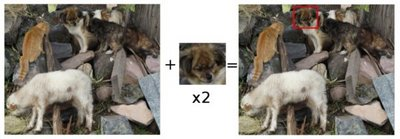
\includegraphics[scale=1]{figures/tm1.jpg}
\caption{Prikaz izvorne slike, slike predloška i krajnjeg rezultata
metode usporedbe predloškom}
\label{fig:tm1.jpg}
\end{figure}

Identificiranje odgovarajućeg područja, radi se uspoređivanjem slike
predloška s izvornom slikom. Pomicanjem predloška piksel po piksel po
izvornoj slici s lijeva na desno, od gore prema dolje kao što je
prikazano na slici~\ref{fig:tm2.jpg}. Na svakoj lokaciji, računa se
vrijednost koja predstavlja koliko dobro predložak odgovara izvornoj
slici, odnosno koliko su slični.

\begin{figure}[h]
\centering
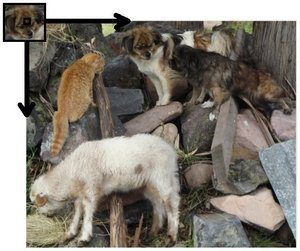
\includegraphics[scale=0.5]{figures/tm2.jpg}
\caption{Prikaz pomicanja predloška po izvornoj slici}
\label{fig:tm2.jpg}
\end{figure}

Za svaku lokaciju piksela u predlošku T preko slike I, pohranjuju se
vrijednosti u matricu rezultata R. Svaka lokacija (x, y) u matrici R
sadrži vrijednost koja govori koliko je na toj lokaciji predložak
sličan izvornoj slici. 

Slika~\ref{fig:tm3.jpg} prikazuje rezultate R pomicanja predloška po
izvornoj slici. Korištena metoda je \texttt{TM\_CCORR\_NORMED}.
Najsvjetlija mjesta pokazuju odgovarajuće vrijednosti. Kao što se vidi,
mjesto obilježeno crvenim krugom je ono s najvišom vrijednosti. U praksi
se za pronalazak najvećih odnosno najmanjih vrijednosti koristi funkcija
\texttt{minMaxLoc} ovisno o metodi koja se koristi.


\begin{figure}[h]
\centering
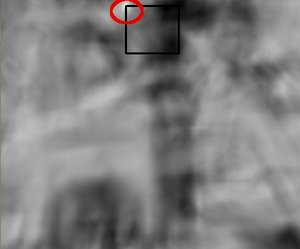
\includegraphics[scale=0.8]{figures/tm3.jpg}
\caption{Prikaz matrice rezultata R nakon usporedbe s predloškom}
\label{fig:tm3.jpg}
\end{figure}

OpenCV funkcija \texttt{matchTemplate} sadrži nekoliko metoda za
računanje rezultantne matrice. Slijede njihove jednadžbe:
\begin{itemize}
    \item \textbf{CV\_TM\_SQDIFF} 
    \begin{equation}
         R\left ( x,y \right )= \sum_{{x}',{y}'} (T({x}',{y}')-I\left ( x+{x}',y+{y}' \right ))^{2}
	\end{equation}
    \item \textbf{CV\_TM\_SQDIFF\_NORMED} 
    \begin{equation}
     R\left ( x,y \right )= \frac{\sum_{{x}',{y}'}(T({x}',{y}' - I\left ( x+{x}',y+{y}' \right ))^{2}}{\sqrt{\sum_{{x}',{y}'}T({x}',{y}')^{2}\cdot \sum_{{x}',{y}'}I\left ( x+{x}',y+{y}' \right ))^{2}}}
    \end{equation}
    \item \textbf{CV\_TM\_CCORR} 
    \begin{equation}
     R\left ( x,y \right )= \sum_{{x}',{y}'} (T({x}',{y}')\cdot I\left ( x+{x}',y+{y}' \right ))^{2}
    \end{equation}
    \item \textbf{CV\_TM\_CCORR\_NORMED} 
    \begin{equation}
     R\left ( x,y \right ) = \frac{\sum_{{x}',{y}'}(T({x}',{y}')\cdot I\left ( x+{x}',y+{y}' \right ))^{2}}{\sqrt{\sum_{{x}',{y}'}T({x}',{y}')^{2}\cdot \sum_{{x}',{y}'}I\left ( x+{x}',y+{y}' \right ))^{2}}}
    \end{equation}
    \item \textbf{CV\_TM\_CCOEFF} 
     \begin{equation}
      R\left ( x,y \right )= \sum_{{x}',{y}'} ({T}'({x}',{y}')\cdot I\left ( x+{x}',y+{y}' \right ))^{2}
     \end{equation}
     gdje je:
    \begin{equation}
     {T}'({x}',{y}')=T({x}',{y}')-1/(w\cdot h)\cdot \sum_{{x}'',{y}''}T({x}'',{y}'')
    \end{equation}
    \begin{equation}
      I\left ( x+{x}',y+{y}' \right )=I\left ( x+{x}',y+{y}' \right )- \sum_{{x}'',{y}''}I\left ( x+{x}'',y+{y}'' \right ))^{2}
      \end{equation}
    \item \textbf{CV\_TM\_CCOEFF\_NORMED} 
    \begin{equation}
      R\left ( x,y \right )= \frac{ \sum_{{x}',{y}'}({T}'({x}',{y}')\cdot {I}'\left ( x+{x}',y+{y}' \right ))^{2}}{\sqrt{\sum_{{x}',{y}'}{T}'({x}',{y}')^{2}\cdot \sum_{{x}',{y}'}{I}'\left ( x+{x}',y+{y}' \right ))^{2}}}
    \end{equation}
\end{itemize}


\newpage
\subsubsection{Primjer korištenje funkcije \texttt{matchTemplate} } % (fold)
\label{ssub:Primjer korištenje funkcije }

Slijedi primjer korištenja funkcije \texttt{matchTemplate} za pronalazak
predloška na učitanoj slici.

1. Uključivanje potrebnih zaglavlja i deklaracija varijabli za spremanje
slika i naziv prozora.
\begin{lstlisting}[label=lst1,caption={}]
#include "opencv2/highgui/highgui.hpp"
#include "opencv2/imgproc/imgproc.hpp"
#include <iostream>
#include <stdio.h>
using namespace std;
using namespace cv;

void main () {
Mat img; Mat templ; Mat result;
char* image_window = "Source Image";
char* result_window = "Result window";
int match_method;
\end{lstlisting}

2. Učitavanje izvorne slike i slike predloška preko argumenata predanih
programu.
\begin{lstlisting}[caption={}]
img = imread( argv[1], 1 );
templ = imread( argv[2], 1 );
match_method = argv[3];
\end{lstlisting}

3. Kreiranje prozora za prikaz učitane slike i slike rezultata.
\begin{lstlisting}[caption={}]
namedWindow( image_window, CV_WINDOW_AUTOSIZE );
namedWindow( result_window, CV_WINDOW_AUTOSIZE );
\end{lstlisting}

4. Računanje veličine matrice rezultata i njeno kreiranje.
\begin{lstlisting}[caption={}]
int result_cols =  img.cols - templ.cols + 1;
int result_rows = img.rows - templ.rows + 1;
result.create( result_cols, result_rows, CV_32FC1 )
\end{lstlisting}

5. Pozivanje funkcije matrice rezultata i predavanje potrebnih
argumenata: izvorna slika, slika predloška, matrica rezultata, broj
metode.
\begin{lstlisting}[caption={}]
matchTemplate( img, templ, result, match_method );
\end{lstlisting}

6. Normaliziranje rezultata.
\begin{lstlisting}[caption={}]
normalize( result, result, 0, 1, NORM_MINMAX, -1, Mat() );
\end{lstlisting}

7. Kreiranje varijabli za pronalazak maksimalne i minimalne vrijednost i
lokacije te pozivanje funkcije za pronalazak istih.
\begin{lstlisting}[caption={}]
double minVal; double maxVal; Point minLoc; Point maxLoc;
Point matchLoc;
minMaxLoc( result, &minVal, &maxVal, &minLoc, &maxLoc, Mat() );
\end{lstlisting}

8. Iscrtavanje pravokutnika oko pronađenih lokacija te prikaz prozora
izvorne slike i rezultata.
\begin{lstlisting}[caption={}]
rectangle( img_display, matchLoc, Point( matchLoc.x + templ.cols , matchLoc.y + templ.rows ), Scalar::all(0), 2, 8, 0 );
rectangle( result, matchLoc, Point( matchLoc.x + templ.cols , matchLoc.y + templ.rows ), Scalar::all(0), 2, 8, 0 );
imshow( image_window, img_display );
imshow( result_window, result );

waitKey(0);
}
\end{lstlisting}
% subsubsection Primjer korištenje funkcije tt (end)

% subsection Algoritam usporedbe predloškom (end)
\subsection{Prepoznavanje znakovlja u pokretnoj slici} % (fold)

Pokretna slika odnosno video je zapravo niz statičnih slika 
koje se izmjenjuju određenom brzinom. Time se dobiva iluzija da se 
radi o pokretnoj slici. Činjenica da se pokretna slika sastoji od
niza statičnih slika olakšava prepoznavanje 
znakova jer se iste metode mogu primjeniti i na pokretnu sliku. 
Programi obično učitavaju svaku sliku ili sličicu (engl. \textit{frame}) i izvršavaju algoritam za pronalazak znaka.

% section Tehnologija i teorija (end)
